\documentclass[preprint,12pt]{elsarticle}

\usepackage{amsmath,amssymb}
\usepackage{booktabs}
\usepackage{graphicx}
\usepackage{multirow}
\usepackage{array}
\usepackage{xcolor}
\usepackage{hyperref}

\journal{Medical Image Analysis}

\begin{document}

\begin{frontmatter}

\title{SafeRefine: Certification Frontiers for Risk-Controlled Segmentation Refinement}

\author[inst1]{Author One}
\author[inst1]{Author Two}
\author[inst1]{Author Three}
\address[inst1]{Institution, City, Country}

\begin{abstract}
Medical image segmentation pipelines often refine a host prediction after a
model produces a mask. The key deployment question is not only whether
refinement improves average Dice, but when a proposed intervention must be
refused because the calibration evidence does not support its case-level risk.
We propose SafeRefine, a model-agnostic calibration framework that wraps a host
segmenter and a portfolio of candidate actions including an exact host-fallback
action. A calibrated controller accepts a non-host action only when its risk
score passes a learned threshold and the selected action-threshold pair
satisfies finite-sample upper-confidence constraints on harmed-rate, large-drop
rate, and mean harm; otherwise it preserves the host and outputs a single
operational mask.
We evaluate SafeRefine across dermoscopy, endoscopy, and MRI with GraphSeg and
UNet hosts, hand-crafted action zoos, and a stress portfolio in which an
independently trained UNet is an alternative action over a GraphSeg host. Under
the primary tail-risk contract,
the controller returns the host in all eight settings: the tested actions are
not certifiable with the available calibration evidence. This refusal persists
under empirical-Bernstein and Clopper--Pearson bounds and a nested
low-multiplicity variant. We then map the certification frontier: relaxing the
moderate-drop budget certifies some non-host actions, but a severe-tail
constraint on $g<-0.20$ failures returns all settings to the host.
As a positive control, a synthetic artifact-removal task shows that SafeRefine
certifies and accepts a low-risk refiner. SafeRefine thus frames
refinement as calibrated deployment-time refusal: change a host mask only when
finite-sample evidence supports the risk of the intervention.
\end{abstract}

\begin{keyword}
medical image segmentation \sep certification frontier \sep conformal risk control
\sep post-processing \sep host fallback \sep model-agnostic refinement
\end{keyword}

\end{frontmatter}

\section{Introduction}

Medical image segmentation systems are rarely deployed as raw neural-network
outputs alone. Predictions may be smoothed, cleaned, topology-corrected,
refined by a secondary model, or adjusted by a shape prior. These refinements
are attractive because they can improve average overlap metrics, remove
implausible components, and restore clinically meaningful structures. However,
an unconditional refinement rule creates a deployment risk: the same operation
that improves one case can damage another. In medical imaging, this matters
because case-level harm, not only population-level average Dice, is central to
clinical reliability.

This work starts from a simple observation. A trained host segmenter already
provides a valid prediction. Any refinement should therefore be treated as an
intervention on top of that prediction, not as an unconditional replacement. A
risk-controlled refinement system should answer three questions for each image:
should the host be kept unchanged, which refinement action should be used, and
how much case-level harm is introduced by this decision rule?

We propose SafeRefine, a model-agnostic safety layer for medical segmentation
refinement. The framework takes a host mask or logits and a set of candidate
actions. Candidate actions may include morphology, component filtering,
probability smoothing, graph-membrane refinement, or learned refiners.
The action set always includes the host action, which returns the original host
prediction exactly. A calibration split is used to select an action and a risk
threshold. At test time, the selected action is applied only if its measured
risk is below the threshold; otherwise the output is exactly the host mask.

SafeRefine converts arbitrary refinement operators into a deployable acceptance
policy with explicit harm accounting. This changes the empirical question from
``does a fixed refiner improve mean Dice?'' to ``when should a proposed
refinement be accepted, and when should the host be preserved?'' The primary
evidence is therefore safety value: how much harm and worst-case degradation are
prevented when a calibrated intervention policy replaces unconditional
refinement.

Our contributions are:
\begin{enumerate}
    \item We formulate medical segmentation refinement as calibrated
    acceptance/rejection of candidate refiners over a host-preserving action
    portfolio.
    \item We introduce a tail-risk-controlled acceptance policy that optimizes
    calibrated utility subject to upper-confidence constraints on harmed-rate,
    large-drop rate, and mean harm, and explicitly separate this full
    conservative mode from a Bernoulli tail-risk variant.
    \item We evaluate geometry-aware, uncertainty-based, and learned
    quality-risk scores as candidate gating signals, without assuming that any
    single score is universally optimal.
    \item We evaluate the same controller across medical segmentation
    datasets, host families, morphology-only and broader refiner-zoo action
    sets, and a three-setting stress portfolio in which an independently trained
    UNet is added as an alternative (standalone-segmenter) action over a
    GraphSeg host.
    \item We report safety-first quantities: mean gain, mean harm, worst drop,
    harmed-rate, large-drop rate, tail harm, revert-rate, and bootstrap
    confidence intervals.
\end{enumerate}

\section{Related Work}

\subsection{Post-processing and mask refinement}

Classical post-processing such as morphology, connected-component filtering,
conditional random fields, active contours, and level-set methods remains
common in medical segmentation, including strong engineering baselines such as
nnU-Net that combine robust model design with simple post-processing
\cite{isensee2021nnunet}. Modern learned refiners, including boundary
correction modules, class-agnostic mask refinement, point-based refinement, and
diffusion-based refinement, can further improve mask quality
\cite{zheng2015crfrnn,yuan2020segfix,cheng2020cascadepsp,kirillov2020pointrend,segrefiner2023}.
These methods usually ask whether a refinement operator improves average
performance. SafeRefine is orthogonal: it asks whether a candidate refinement
should be accepted for a given image and provides the host prediction as an
exact fallback.

\subsection{Graph and geometry-aware refinement}

Graph-based medical refinement methods use superpixels, grid graphs, dynamic
neighborhoods, or graph neural networks to propagate local structure and
correct segmentation outputs
\cite{soberanis2020uncertainty,demir2021dynamicgraph}. This literature
motivates geometry-aware candidate actions and risk scores, but most prior
graph-refinement systems are fixed predictors. Our controller treats graph or
geometry mechanisms as actions in a portfolio. The novelty claim is not graph
message passing by itself; it is the calibrated intervention policy around
arbitrary refiners.

\subsection{Conformal prediction and risk control}

Conformal prediction and conformal risk control provide finite-sample tools for
calibrating prediction sets, uncertainty maps, and risk-bounded outputs
\cite{vovk2005algorithmic,angelopoulos2021gentle,romano2019conformal,bates2021distributionfree,angelopoulos2024crc}.
These ideas are increasingly used for segmentation
\cite{mossina2024conformal,morphological2025conformal}.
SafeRefine is adjacent but has a different operational target. It does not
output an uncertainty set or a coverage map. It outputs one segmentation mask
selected from an action portfolio: either the host or an accepted refinement.
The closest conceptual connection is risk-controlled decision making, but our
focus is medical segmentation refinement with exact host fallback and harm/gain
accounting.

\subsection{Failure detection, rejection, and deferral}

Medical segmentation reliability work often estimates uncertainty, detects
failures, flags uncertain cases, or defers regions to humans or expert models
\cite{gal2016dropout,kendall2017uncertainties,baumgartner2019phiseg,roy2019quicknat,mehrtash2020confidence,jungo2020analyzing,deferredseg2026}.
Selective prediction and reject-option classification similarly study when a
prediction should not be emitted
\cite{chow1970optimum,elyaniv2010foundations,geifman2017selective}.
SafeRefine instead performs autonomous post-hoc acceptance or rejection of
candidate refinement. Reverting to the host is not a request for manual review;
it is a deterministic deployment decision preserving the original model output.

Because one candidate in our stress portfolio is an alternative standalone
segmenter rather than a host-conditioned correction, SafeRefine also connects to
model selection, cascades, and mixture-of-experts schemes that route each input
to one of several predictors \cite{isensee2021nnunet,cheng2020cascadepsp}. The
difference is the objective: SafeRefine does not select the most accurate model,
but certifies whether replacing the host is supported under explicit case-level
harm budgets, and defaults to the host whenever it is not.

\section{Method}

\subsection{Host-preserving action portfolio}

Let a host segmentation model produce logits or a binary mask for image $x$.
Denote the host prediction by $h(x)$. A candidate action set is
\begin{equation}
    \mathcal{A}(x) = \{\mathrm{host}, r_1(h,x), \ldots, r_K(h,x)\}.
\end{equation}
The host action returns $h(x)$ exactly. Each $r_k$ is a candidate refiner. In
the current experiments, actions include morphology with multiple kernel sizes,
connected-component and hole-fill operations, probability smoothing, bilateral
smoothing, and graph/geometry-derived refiners.

\subsection{Gain, harm, and policy class}

For image $i$, action $a$, ground truth $y_i$, and metric $m(\cdot,\cdot)$, we
define the gain relative to the host:
\begin{equation}
    g_i(a) = m(a(x_i), y_i) - m(h(x_i), y_i).
\end{equation}
The non-negative harm is
\begin{equation}
    \ell_i(a) = \max(0, -g_i(a)).
\end{equation}

The action policy is parameterized by an action $a$ and threshold $\tau$:
\begin{equation}
    \pi_{a,\tau}(x) =
    \begin{cases}
        a(x), & \rho_a(x) \leq \tau,\\
        h(x), & \rho_a(x) > \tau,
    \end{cases}
\end{equation}
where $\rho_a(x)$ is an action-specific risk score. The host action is always
feasible and has zero gain and zero harm relative to itself.

We distinguish two policy classes. The primary policy used in the main results
selects one action and one threshold on calibration, then either applies that
action or falls back to the host. This is a conservative acceptance mode. As a
methodology stress test, we also evaluate true per-image portfolio selection:
a meta-training split fits predicted-gain and predicted-harm models, a
separate calibration split selects a risk threshold, and each test image
chooses the feasible action with highest predicted utility or returns the host
if no action has positive predicted utility.

\paragraph{Exact fallback property.}
For any image $x$, if the selected non-host action fails the risk threshold, or
if calibration selects the host action, then $\pi(x)=h(x)$ exactly. Therefore,
the policy class contains a deployment-safe identity policy independently of
the candidate refiners. This is a simple property, but it is central to the
method: unsafe or uncertified refiners can be placed in the portfolio without
forcing them to modify the final segmentation.

\subsection{Harm-aware calibration}

Policies are selected on a calibration split. Among feasible policies, we
maximize
\begin{equation}
    U(\pi) = \frac{1}{n}\sum_i g_i(\pi) -
    \beta_{\mathrm{harm}}\frac{1}{n}\sum_i \ell_i(\pi).
\end{equation}
This objective prevents a policy from being selected solely because it improves
the mean while introducing large case-level degradation.

\subsection{CRC-style feasibility and controlled risk}

For each action-threshold pair, we estimate three calibration risks: the
harmed-rate, the large-drop rate $\Pr(g<-0.05)$, and the mean harm
$\mathbb{E}\max(0,-g)$. A Hoeffding upper confidence bound with a union
correction over tested thresholds and controlled risk constraints is computed:
\begin{equation}
    \widehat{R}_{\mathrm{ucb}} =
    \widehat{R} + s_R\sqrt{\frac{\log(MR/\delta)}{2n}},
\end{equation}
where $M$ is the number of tested action-threshold candidates, $R$ is the
number of simultaneously controlled risks, and $\delta$ is the total failure
probability allocated to the policy selection step. Equivalently, the bound
uses an equal split $\delta/(MR)$ across all action-threshold and risk
constraints. For Bernoulli risks, $s_R=1$; for mean harm, $s_R$ is the bounded
harm scale used for the Hoeffding correction. Since Dice lies in $[0,1]$, the
harm $\max(0,-g)$ is also bounded in $[0,1]$, and we use this range for the
primary mean-harm bound. The primary tail-risk-controlled policy is feasible
only if
\begin{align}
    \widehat{\Pr(g<0)}_{\mathrm{ucb}} &\leq \alpha, \\
    \widehat{\Pr(g<-0.05)}_{\mathrm{ucb}} &\leq \gamma, \\
    \widehat{\mathbb{E}\max(0,-g)}_{\mathrm{ucb}} &\leq \eta.
\end{align}
In the primary experiments we use $\alpha=0.25$, $\gamma=0.10$, and
$\eta=0.02$. These are calibration risk budgets for candidate intervention
acceptance, not clinical safety guarantees. If no non-host policy is feasible,
the controller returns the host.

\paragraph{Proposition 1 (finite-sample host-fallback risk guarantee).}
Assume that the calibration cases are exchangeable with future deployment
cases, that each controlled risk variable is bounded in $[0,s_R]$, and that
the action-threshold candidates and risk constraints tested by the calibration
procedure are included in the union correction above. With probability at
least $1-\delta$ over the calibration sample, every tested
action-threshold-risk triple has true risk no larger than its reported
Hoeffding upper bound. Consequently, any selected non-host policy satisfying
the three feasibility inequalities has harmed-rate, large-drop rate, and mean
harm no larger than $(\alpha,\gamma,\eta)$ under the calibration/deployment
distribution. If no non-host policy satisfies the inequalities, SafeRefine
selects the host action and therefore has exactly zero gain and zero harm
relative to the host output on every case.

\paragraph{Proof sketch.}
For a fixed action-threshold-risk triple, Hoeffding's inequality bounds the
probability that the true bounded risk exceeds
$\widehat{R}+s_R\sqrt{\log(MR/\delta)/(2n)}$ by at most $\delta/(MR)$. A union
bound over the $M$ tested action-threshold candidates and $R$ controlled risks
gives simultaneous coverage with probability at least $1-\delta$. The selected
policy is one of these tested candidates, so feasibility of its upper bounds
implies feasibility of its true risks on the same exchangeable population. The
host fallback statement follows directly from the exact host action
$\pi(x)=h(x)$, for which $g=0$ and $\ell=0$ for every image.

We additionally evaluate a Bernoulli tail-risk primary variant that applies
the same calibration search but constrains only harmed-rate and large-drop
rate. This diagnostic variant separates the effect of the continuous mean-harm
bound from the two event-risk constraints. It is not used to weaken the primary
claim; it asks whether non-host rejection is driven only by the mean-harm UCB
or also by the finite-sample evidence for harmful and large-drop events.

Finally, we evaluate a nested-selection stress test. The first split selects a
candidate action using harm-aware utility; the second split calibrates only the
thresholds for that selected action; the third split is held out for testing.
This reduces the multiplicity term from the full action-threshold portfolio to
the thresholds of one selected action. In this nested variant we use
$\epsilon=0.01$ for the harmed event, retain the large-drop event
$g<-0.05$, and require positive calibration utility for non-host intervention;
otherwise the policy falls back to the host.

Because controlling the frequency of $g<-0.05$ drops does not preclude rare
catastrophic failures, we also run a severe-tail sensitivity analysis with an
additional Bernoulli constraint on $\Pr(g<-0.20)$. This analysis is not used to
claim a new primary operating point; it tests how much stricter the evidence
requirement becomes when very large case-level degradation is explicitly
included in the acceptance contract.

The controlled event is image-level degradation beyond a tolerance $\epsilon$:
\begin{equation}
    Z_i(\pi) = \mathbb{1}\{g_i(\pi) < -\epsilon\}.
\end{equation}
In the experiments we use $\epsilon=0$, so a harmful refinement is any selected
action whose Dice is lower than the host Dice on that image. Large-drop and
mean-harm constraints make the policy sensitive to tail risk, not only to the
frequency of small negative changes. We also report utility-oriented
single-risk analyses with a non-zero harmed-rate budget; these are exploratory
operating points for quantifying available gain and residual harm, not the
primary safety claim.

Because the controller searches over many actions, thresholds, and risk
constraints, the confidence level is divided across the full set of tested
action-threshold-risk triples in the Hoeffding bound.
Under the usual exchangeability assumption between calibration and deployment
samples, the selected policy has calibration harmed-rate upper bound at most
the requested budget, and analogously satisfies the large-drop and mean-harm
upper-bound constraints, with the stated confidence after accounting for this
multiple selection. This is a finite-sample calibration statement for the
acceptance policy; it is not claimed as a new conformal theorem.

We also run a bound-sensitivity analysis using empirical Bernstein bounds and
Clopper--Pearson upper bounds for the two Bernoulli risks. For mean harm, the
sensitivity analysis keeps the same bounded empirical-Bernstein/Hoeffding style
upper bound because the risk is continuous rather than Bernoulli. These
analyses are reported to distinguish true non-certifiability from excessive
conservatism of one particular finite-sample bound.

We keep a zero-budget identity setting only as a fallback lower bound. With
finite calibration data and a Hoeffding upper bound, any non-host policy with a
non-zero uncertainty term generally has a positive upper bound even if no harm
is observed; under a zero harmed-rate budget, the host action is therefore the
only policy that can always satisfy the constraint exactly. This zero-budget
mode is reported to verify the fallback contract, not as an empirical performance
achievement.

SafeRefine is also distinct from selective prediction. Selective prediction
decides whether to accept or reject a model prediction. SafeRefine decides
whether to accept a proposed segmentation intervention. Rejection is not
abstention or referral to a human; it returns the host segmentation exactly.
The output remains a single usable segmentation mask in all cases.

The novelty is therefore not a new concentration inequality, nor the claim that
morphology-based refinement is itself new. The contribution is to reframe
post-hoc medical segmentation refinement as a calibrated intervention problem:
given an already accepted host mask, the controller may alter that mask only
when a finite-sample calibration rule supports the case-level harm of the
intervention; otherwise it falls back exactly to the host and accounts for harm
at the image or patient level.

\subsection{Geometry-aware risk scores}

We evaluate three risk scores. The simplest is the fraction of pixels changed
relative to the host:
\begin{equation}
    \rho_{\mathrm{changed}}(x,a) =
    \frac{1}{|\Omega|}\sum_{p\in\Omega}
    \mathbb{1}\{a(x)_p \neq h(x)_p\}.
\end{equation}
The geometry-aware score augments this with area, centroid, and topology-like
component changes:
\begin{equation}
    \rho_{\mathrm{geom}} =
    \rho_{\mathrm{changed}}
    + \Delta_{\mathrm{area}}
    + 0.25\Delta_{\mathrm{centroid}}
    + 0.01\Delta_{\mathrm{components}}.
\end{equation}
We also evaluate $\rho_{\mathrm{changed}} + \rho_{\mathrm{geom}}$. These scores
are intentionally simple and interpretable: they measure how much a refiner
changes the host and whether the change is geometrically large.
They should not be read as a claim that geometry, changed-area, uncertainty, or
quality estimates are stable universal predictors of refinement harm. SafeRefine
is a calibration framework over candidate risk scores; the simple scores used
here are interpretable but imperfect signals whose limitations are measured in
the experiments.

\begin{figure*}[t]
    \centering
    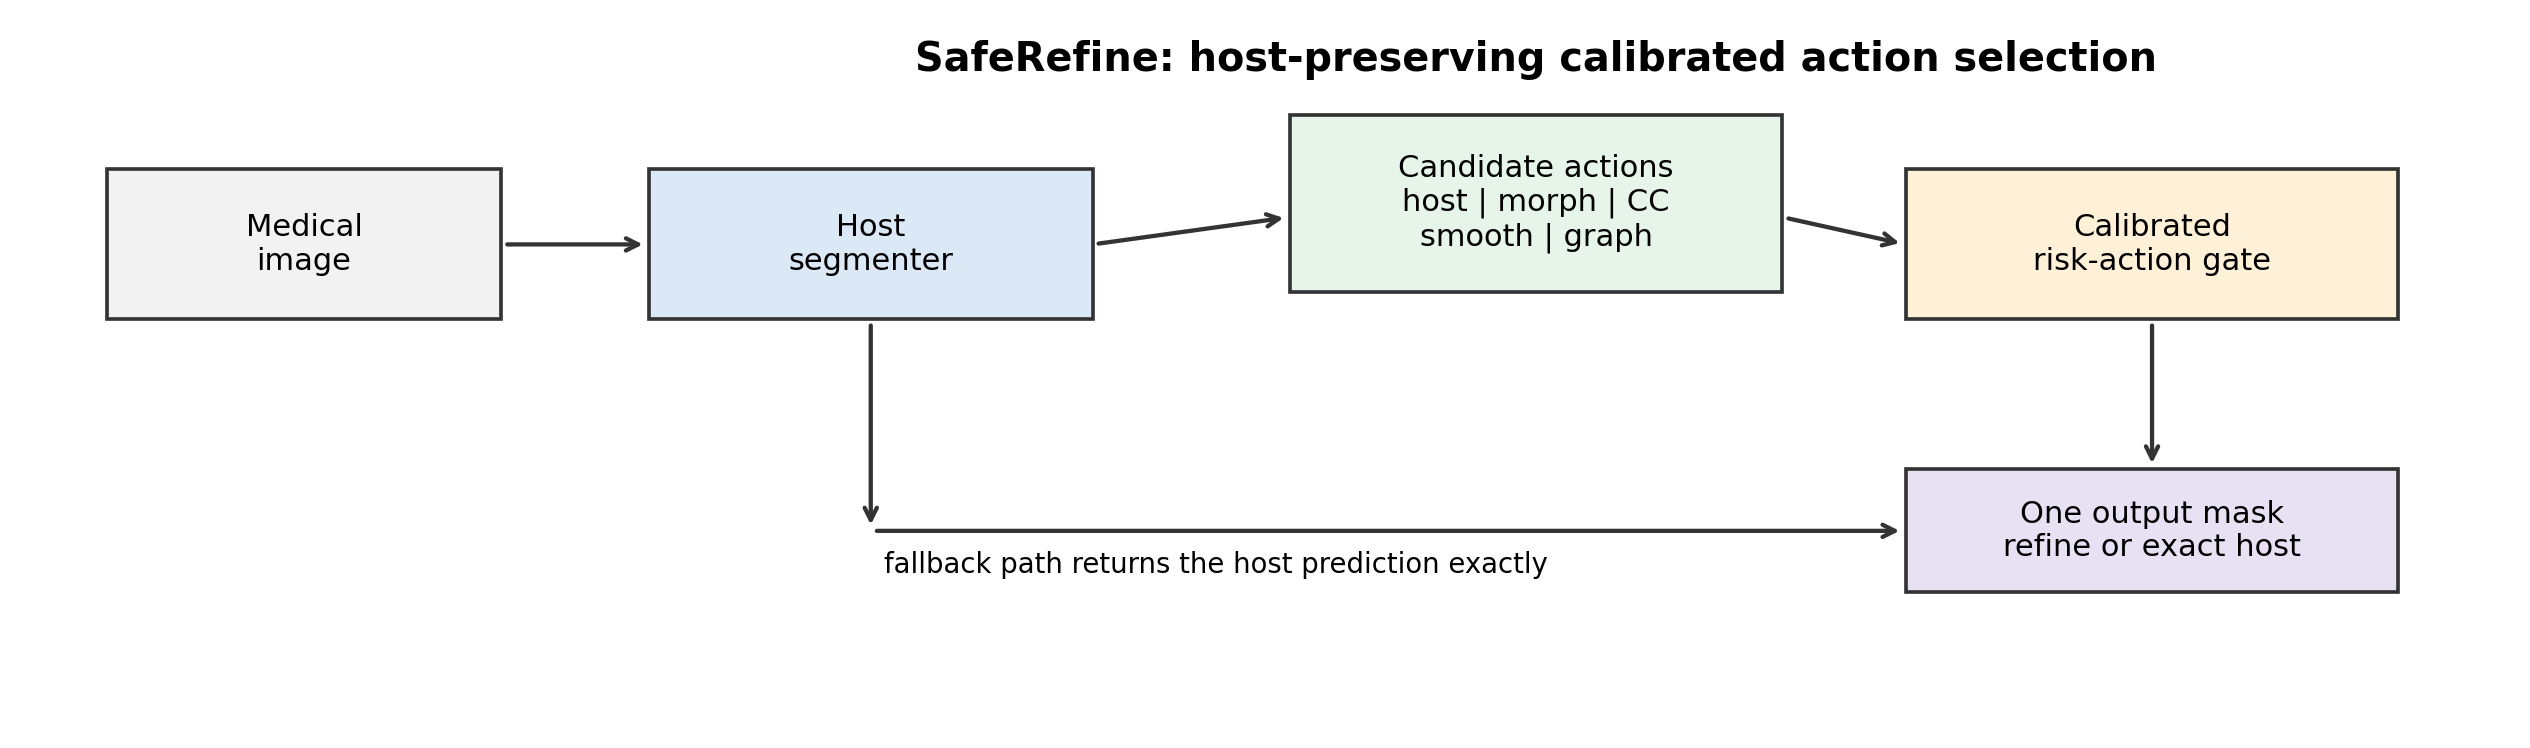
\includegraphics[width=0.95\textwidth]{figures/fig_method_schematic.png}
    \caption{SafeRefine wraps an existing host segmenter and a portfolio of
    candidate refiners. The host action is always available and returns the
    original prediction exactly. The calibrated controller applies a refinement
    only when its risk score is below the selected threshold.}
    \label{fig:method}
\end{figure*}

\section{Experiments}

\subsection{Datasets and host models}

We evaluate binary medical segmentation tasks across dermoscopy, endoscopy, and
MRI. The final internally consistent binary runs use ISIC 2018 Task 1 lesion
segmentation \cite{codella2019skin}, PH2 lesion segmentation
\cite{mendonca2013ph2}, Kvasir-SEG polyp segmentation \cite{jha2020kvasir},
MSD Heart left-atrium MRI segmentation \cite{antonelli2022msd}, and an
external polyp stress set aggregated from official polyp benchmarks. All images
and masks are resized to $352\times352$. Masks are binarized as foreground
versus background using a positive-label threshold after nearest-neighbor mask
resizing.

\begin{table*}[t]
\centering
\small
\caption{Dataset sizes after preprocessing. Two-dimensional dermoscopy and
endoscopy datasets use image-level splits because patient identifiers are not
available in the staged files. MSD Heart MRI uses patient-level splits.}
\label{tab:dataset_protocol}
\begin{tabular}{llll}
\toprule
Dataset & Cases after preprocessing & Split & Split unit \\
\midrule
ISIC 2018 Task 1 & 3694 images & 2594 / 100 / 1000 & image \\
PH2 & 200 images & 140 / 30 / 30 & image \\
Kvasir-SEG & 1000 images & 700 / 150 / 150 & image \\
MSD Heart MRI & 20 volumes, 1417 slices & 981 / 214 / 222 slices & patient \\
External polyp stress set & 2248 images & 1232 / 218 / 798 & image \\
\bottomrule
\end{tabular}
\end{table*}

For MSD Heart MRI, the patient-level split uses 14 training, 3 validation, and
3 test volumes, yielding 981 training, 214 validation, and 222 test slices
after retaining the annotated atrium region with a two-slice margin. The
external polyp test split contains CVC-300 (60), CVC-ColonDB (380),
ETIS-LaribPolypDB (196), Kvasir (100), and CVC-ClinicDB (62) cases as recorded
in the NPZ identifiers. Host models include GraphSeg/SegFormer-B0-style models
and a dependency-free small UNet. Hosts are trained from scratch within this
repository using the training split and selected by validation performance; the
stored checkpoints used for SafeRefine evaluation are listed in the
reproducibility manifest. The same SafeRefine evaluator is used for all hosts.

\subsection{Candidate action sets}

The baseline action set contains host plus binary morphology at multiple kernel
sizes. The refiner zoo adds close-only, open-only, open-close, hole filling,
largest connected component, largest-component with hole filling, small-object
removal, Gaussian probability smoothing, Gaussian smoothing with component
cleanup, and bilateral probability smoothing. These are deliberately
lightweight, model-agnostic candidate actions. To address the concern that the
portfolio is otherwise dominated by simple post-processing, we also include a
standalone-segmenter stress portfolio in which an independently trained UNet
checkpoint is added as an alternative action over the GraphSeg host on Kvasir,
external polyp, and MSD Heart. We emphasize that in this portfolio the UNet is a
separate segmenter, not a learned refiner: it does not receive the host mask or
host probabilities, and its output is offered to the controller as a candidate
action gated by a host-uncertainty risk score. This setting therefore stresses
the controller as an action/cascade selection diagnostic between a host model
and a stronger standalone model, rather than as a learned host-mask correction.
It is not a broad benchmark of conditioned learned refiners such as
nnU-Net-style cascades, SAM/MedSAM-based mask refinement, SegFix, CascadePSP, or
diffusion refiners. Non-certification should therefore be read as
non-certification of the tested action portfolio, not as evidence that stronger
refiners would fail. Morphology is one candidate action family in a broader
intervention portfolio, not the novelty claim.

\subsection{Protocol}

For each final run, host training, refinement evaluation, policy calibration,
and refiner-zoo evaluation were executed with unique \texttt{mediafinal} tags
to avoid checkpoint/result mixing. The held-out evaluation set is split into
calibration and test halves with calibration fraction 0.5. Bootstrap confidence
intervals use 2000 resamples over test images for the 2D datasets. For MSD
Heart MRI, the reported slice-level metrics are treated as a modality stress
test under patient-disjoint splits, not as patient-level clinical uncertainty
estimates; slice bootstrap intervals are therefore not interpreted as
volume-level confidence intervals. The primary tail-risk policy uses
upper-confidence constraints on harmed-rate, large-drop rate, and mean harm.
Utility analyses with only a non-zero harmed-rate budget are retained as
exploratory operating points for understanding the gain--harm frontier. The
zero-budget identity setting is a fallback lower bound and contract check rather
than an empirical achievement. The primary metrics are host Dice, mean gain over
host, mean harm, worst drop, harmed-rate, revert-rate, large-drop rate, and tail
harm.

Ground truth is used to train and validate the host, to compute candidate
action risks on the calibration split, and to report held-out test metrics. It
is not used to choose actions or thresholds on the test split. Candidate
refiners receive the image, host mask, and/or host probabilities depending on
the action definition, but never the test ground truth. Calibration and test
splits are disjoint; for MRI, they are also patient-disjoint.

\section{Results}

Table~\ref{tab:certification_vs_utility} summarizes how the results should be
read. The primary result is not a Dice-improvement claim: it is a calibrated
refusal result under a conservative tail-risk contract. Certification-frontier,
severe-tail, utility-frontier, and oracle analyses are then used to diagnose
why refinement is rejected, when non-host certification becomes possible, and
how much empirical utility remains outside the certified operating point. This
separation is central: relaxed utility rows are diagnostic operating points, not
a safe-improvement mode.

\begin{table*}[t]
\centering
\small
\caption{Certification versus utility summary. SafeRefine is evaluated first as a finite-sample certification and refusal framework; utility-frontier rows are secondary diagnostics, not a safe-improvement mode.}
\label{tab:certification_vs_utility}
\begin{tabular}{p{0.20\textwidth}p{0.27\textwidth}p{0.15\textwidth}p{0.27\textwidth}}
\toprule
Mode & Safety claim & Non-host certified? & Interpretation \\
\midrule
Primary full tail-risk & Harmed-rate, drop05, and mean-harm upper-confidence constraints. & No & Conservative calibrated refusal; the current refiners are not certifiable under the primary contract. \\
Nested $\epsilon=0.01$ & Reduced multiplicity with action selection separated from threshold calibration. & No & Refusal is not only a union-bound or infinitesimal-Dice artifact. \\
Gamma frontier & Relaxed moderate-drop budget $\Pr(g<-0.05)$. & Sometimes & Certification is budget-dependent; relaxed rows are sensitivity analyses. \\
Severe-tail & Additional constraint on $\Pr(g<-0.20)$. & No & Catastrophic-risk protection returns all settings to the host under current calibration evidence. \\
Utility-frontier & Predefined relaxed diagnostic protocol with measured residual harm. & Mixed & Useful refinements exist, but utility is uneven and uncertified under the primary safety contract. \\
Oracle headroom & Per-image diagnostic upper bound on portfolio utility. & Diagnostic only & The portfolio has headroom, but imperfect risk scores do not reliably recover oracle utility. \\
\bottomrule
\end{tabular}
\end{table*}


\subsection{Fixed refinement can be harmful}

Fixed morphology is not reliably safe. On the external polyp GraphSeg setting,
the best fixed morphology action has mean gain -0.0211, mean harm 0.0524, and
worst drop -0.5093. On ISIC, fixed morphology has positive mean gain but a
worst drop of -0.5228. On MSD Heart MRI with a GraphSeg host, the best fixed
action improves mean Dice by +0.0211 but still has mean harm 0.0499 and worst
drop -0.3276. These are precisely the cases where reporting only mean Dice is
misleading.

\subsection{Primary tail-risk control selects the host under conservative budgets}

Table~\ref{tab:tail_risk_primary_best} reports the primary tail-risk-controlled
SafeRefine policy. Under simultaneous upper-confidence constraints on
harmed-rate, large-drop rate, and mean harm, no tested non-host action is
certified across the final settings. The selected policy is therefore the host
fallback, giving zero measured gain, zero measured harm, zero large-drop rate,
and revert-rate 1.0 on the test split.

This is the main safety statement of the paper: the current candidate refiner
portfolios contain actions that can be useful under relaxed utility operating
points, but they do not satisfy the conservative tail-risk acceptance contract
on the available calibration data. SafeRefine makes that failure to certify visible
and returns the host rather than forcing a risky intervention. For MSD Heart
MRI, the split is patient-level but the metrics are slice-level, so the result
should be read as a conservative modality stress test rather than a definitive
volumetric clinical validation.

\begin{table*}[t]
\centering
\small
\caption{Tail-risk controlled primary SafeRefine policy per setting, selected by calibration utility for compact reporting.}
\label{tab:tail_risk_primary_best}
\begin{tabular}{lllllllll}
\toprule
setting & split & action & gain & harm & harmed\_rate & drop\_gt\_0.05 & worst\_drop & revert\_rate \\
\midrule
ISIC / UNet & image & host & +0.0000 & 0.0000 & 0.000 & 0.000 & +0.0000 & 1.000 \\
Kvasir / GraphSeg & image & host & +0.0000 & 0.0000 & 0.000 & 0.000 & +0.0000 & 1.000 \\
Kvasir / UNet & image & host & +0.0000 & 0.0000 & 0.000 & 0.000 & +0.0000 & 1.000 \\
MSD Heart MRI / GraphSeg & patient & host & +0.0000 & 0.0000 & 0.000 & 0.000 & +0.0000 & 1.000 \\
MSD Heart MRI / UNet & patient & host & +0.0000 & 0.0000 & 0.000 & 0.000 & +0.0000 & 1.000 \\
PH2 / UNet & image & host & +0.0000 & 0.0000 & 0.000 & 0.000 & +0.0000 & 1.000 \\
Polyp ext. / GraphSeg & image & host & +0.0000 & 0.0000 & 0.000 & 0.000 & +0.0000 & 1.000 \\
Polyp ext. / UNet & image & host & +0.0000 & 0.0000 & 0.000 & 0.000 & +0.0000 & 1.000 \\
\bottomrule
\end{tabular}
\end{table*}


Table~\ref{tab:mri_volume_diagnostic} adds a patient-level diagnostic for the
MSD Heart held-out split. Because the primary SafeRefine policy falls back to
the host for MRI, volume-level policy gain and harm are zero by construction;
the table is included to make clear that the MRI cohort contains only three
test volumes and should be interpreted as a modality stress setting rather than
a full volumetric clinical validation.

\begin{table}[t]
\centering
\caption{MSD Heart MRI volume-level diagnostic on the held-out patient split. Values aggregate slice Dice within each of the three test volumes. The fixed learned UNet refiner has large positive average volume gain, but SafeRefine primary falls back to the GraphSeg host, giving zero volume-level harm by construction.}
\label{tab:mri_volume_diagnostic}
\begin{tabular}{lrrrrrl}
\toprule
Policy & Volumes & Mean Dice & Mean gain & Mean harm & Harmed vols & Per-volume values \\
\midrule
GraphSeg host & 3 & 0.334 &  &  &  & 0.455, 0.269, 0.278 \\
Fixed learned UNet refiner & 3 & 0.716 & +0.382 & 0.000 & 0/3 & +0.350, +0.307, +0.490 \\
SafeRefine primary & 3 & 0.334 & +0.000 & 0.000 & 0/3 & +0.000, +0.000, +0.000 \\
\bottomrule
\end{tabular}
\end{table}


Detailed diagnostics are provided in the supplement. In brief, the highest-gain
non-host candidates often have attractive calibration gains, such as +0.0220
Dice for Kvasir-SEG GraphSeg and +0.0155 Dice for MSD Heart MRI GraphSeg, but
their finite-sample upper bounds exceed at least one tail-risk budget. Bound
sensitivity analyses with empirical Bernstein and Clopper--Pearson variants
also select the host. This diagnostic distinction is important: SafeRefine is
rejecting interventions because the available evidence is insufficient for the
stated tail-risk contract, not because the portfolio lacks any utility signal.

\subsection{Standalone-segmenter stress diagnostic}

A second concern is that morphology and smoothing may be too weak an action
portfolio. We therefore add a much stronger candidate: an independently trained
mediafinal UNet checkpoint is offered as an alternative action over the GraphSeg
host on Kvasir, external polyp, and MSD Heart. We stress that this is a
standalone segmenter, not a learned host-mask refiner: the UNet does not receive
the host mask or host probabilities, so the controller is choosing between two
models rather than gating a host-conditioned correction. The action is selected
by a host-uncertainty risk score. The checkpoint pairs are fixed before
SafeRefine calibration; ground truth on the held-out test half is used only for
final evaluation, not for choosing the action or threshold. The standalone
candidate is much stronger on average than the hand-crafted actions: swapping to
it improves fixed test Dice by +0.3729, +0.2074, and +0.4899 on the three
settings. However, the gains are still not uniformly safe. The external polyp
pair has harmed-rate 0.2857 and a worst drop of -0.6678, while the MSD Heart
pair still has a -0.3040 worst slice-level drop despite large mean gain.
Utility-only thresholding continues to select the standalone action in these
settings, whereas the primary SafeRefine contract refuses it and returns the
host. This portfolio is an action-selection stress test, not a benchmark of
conditioned refiners such as MedSAM, SAM-like, CascadePSP, SegFix, or diffusion
models; it addresses the morphology-only concern using a strong learned
candidate across three datasets.

\begin{table}[t]
\centering
\caption{Standalone-segmenter stress portfolio. An independently trained UNet checkpoint is offered as an alternative action over the corresponding GraphSeg host. It is a separate segmenter, not a host-conditioned refiner---it does not receive the host mask or probabilities---and is gated by a host-uncertainty risk score. The standalone candidate improves mean Dice in each setting, but severe case-level degradation remains, and the primary SafeRefine contract falls back to the host.}
\label{tab:learned_refiner_stress}
\begin{tabular}{lrrrrr}
\toprule
Setting & Fixed gain & Mean harm & Worst drop & Harmed & SafeRefine action \\
\midrule
Kvasir / GraphSeg$\rightarrow$UNet & +0.3729 & 0.0007 & -0.0175 & 0.0533 & host \\
Polyp ext. / GraphSeg$\rightarrow$UNet & +0.2074 & 0.0405 & -0.6678 & 0.2857 & host \\
MSD Heart / GraphSeg$\rightarrow$UNet & +0.4899 & 0.0049 & -0.3040 & 0.0323 & host \\
\bottomrule
\end{tabular}
\end{table}


\subsection{Positive-control sanity check}

The host-only primary result raises an important sanity question: can the
controller certify a refiner when a genuinely low-risk useful intervention is
present? We therefore add a non-clinical positive control. Across all
preprocessed datasets, we form a synthetic host by adding a known isolated
square artifact to the ground-truth mask, then include a candidate refiner that
removes exactly that artifact. The controller is evaluated with the same
three-risk Hoeffding correction over $M=1$ candidate threshold and $R=3$ risk
constraints. This experiment is not a clinical segmentation result; it checks
that the calibration machinery accepts a benign useful intervention when the
evidence supports it.

\begin{table}[t]
\centering
\small
\caption{Positive-control artifact-removal experiment. A synthetic host is formed by adding a known isolated square artifact to each ground-truth mask; the candidate refiner removes that artifact. This non-clinical sanity check verifies that SafeRefine certifies a low-risk useful intervention when one exists.}
\label{tab:positive_control}
\begin{tabular}{llllllll}
\toprule
split & $n$ & gain & harm & harmed & drop05 & worst & max UCB \\
\midrule
cal & 4270 & +0.0636 & 0.0000 & 0.000 & 0.000 & +0.0013 & 0.01996 \\
test & 4270 & +0.0671 & 0.0000 & 0.000 & 0.000 & +0.0013 & 0.01996 \\
\bottomrule
\end{tabular}
\end{table}


\begin{figure*}[t]
    \centering
    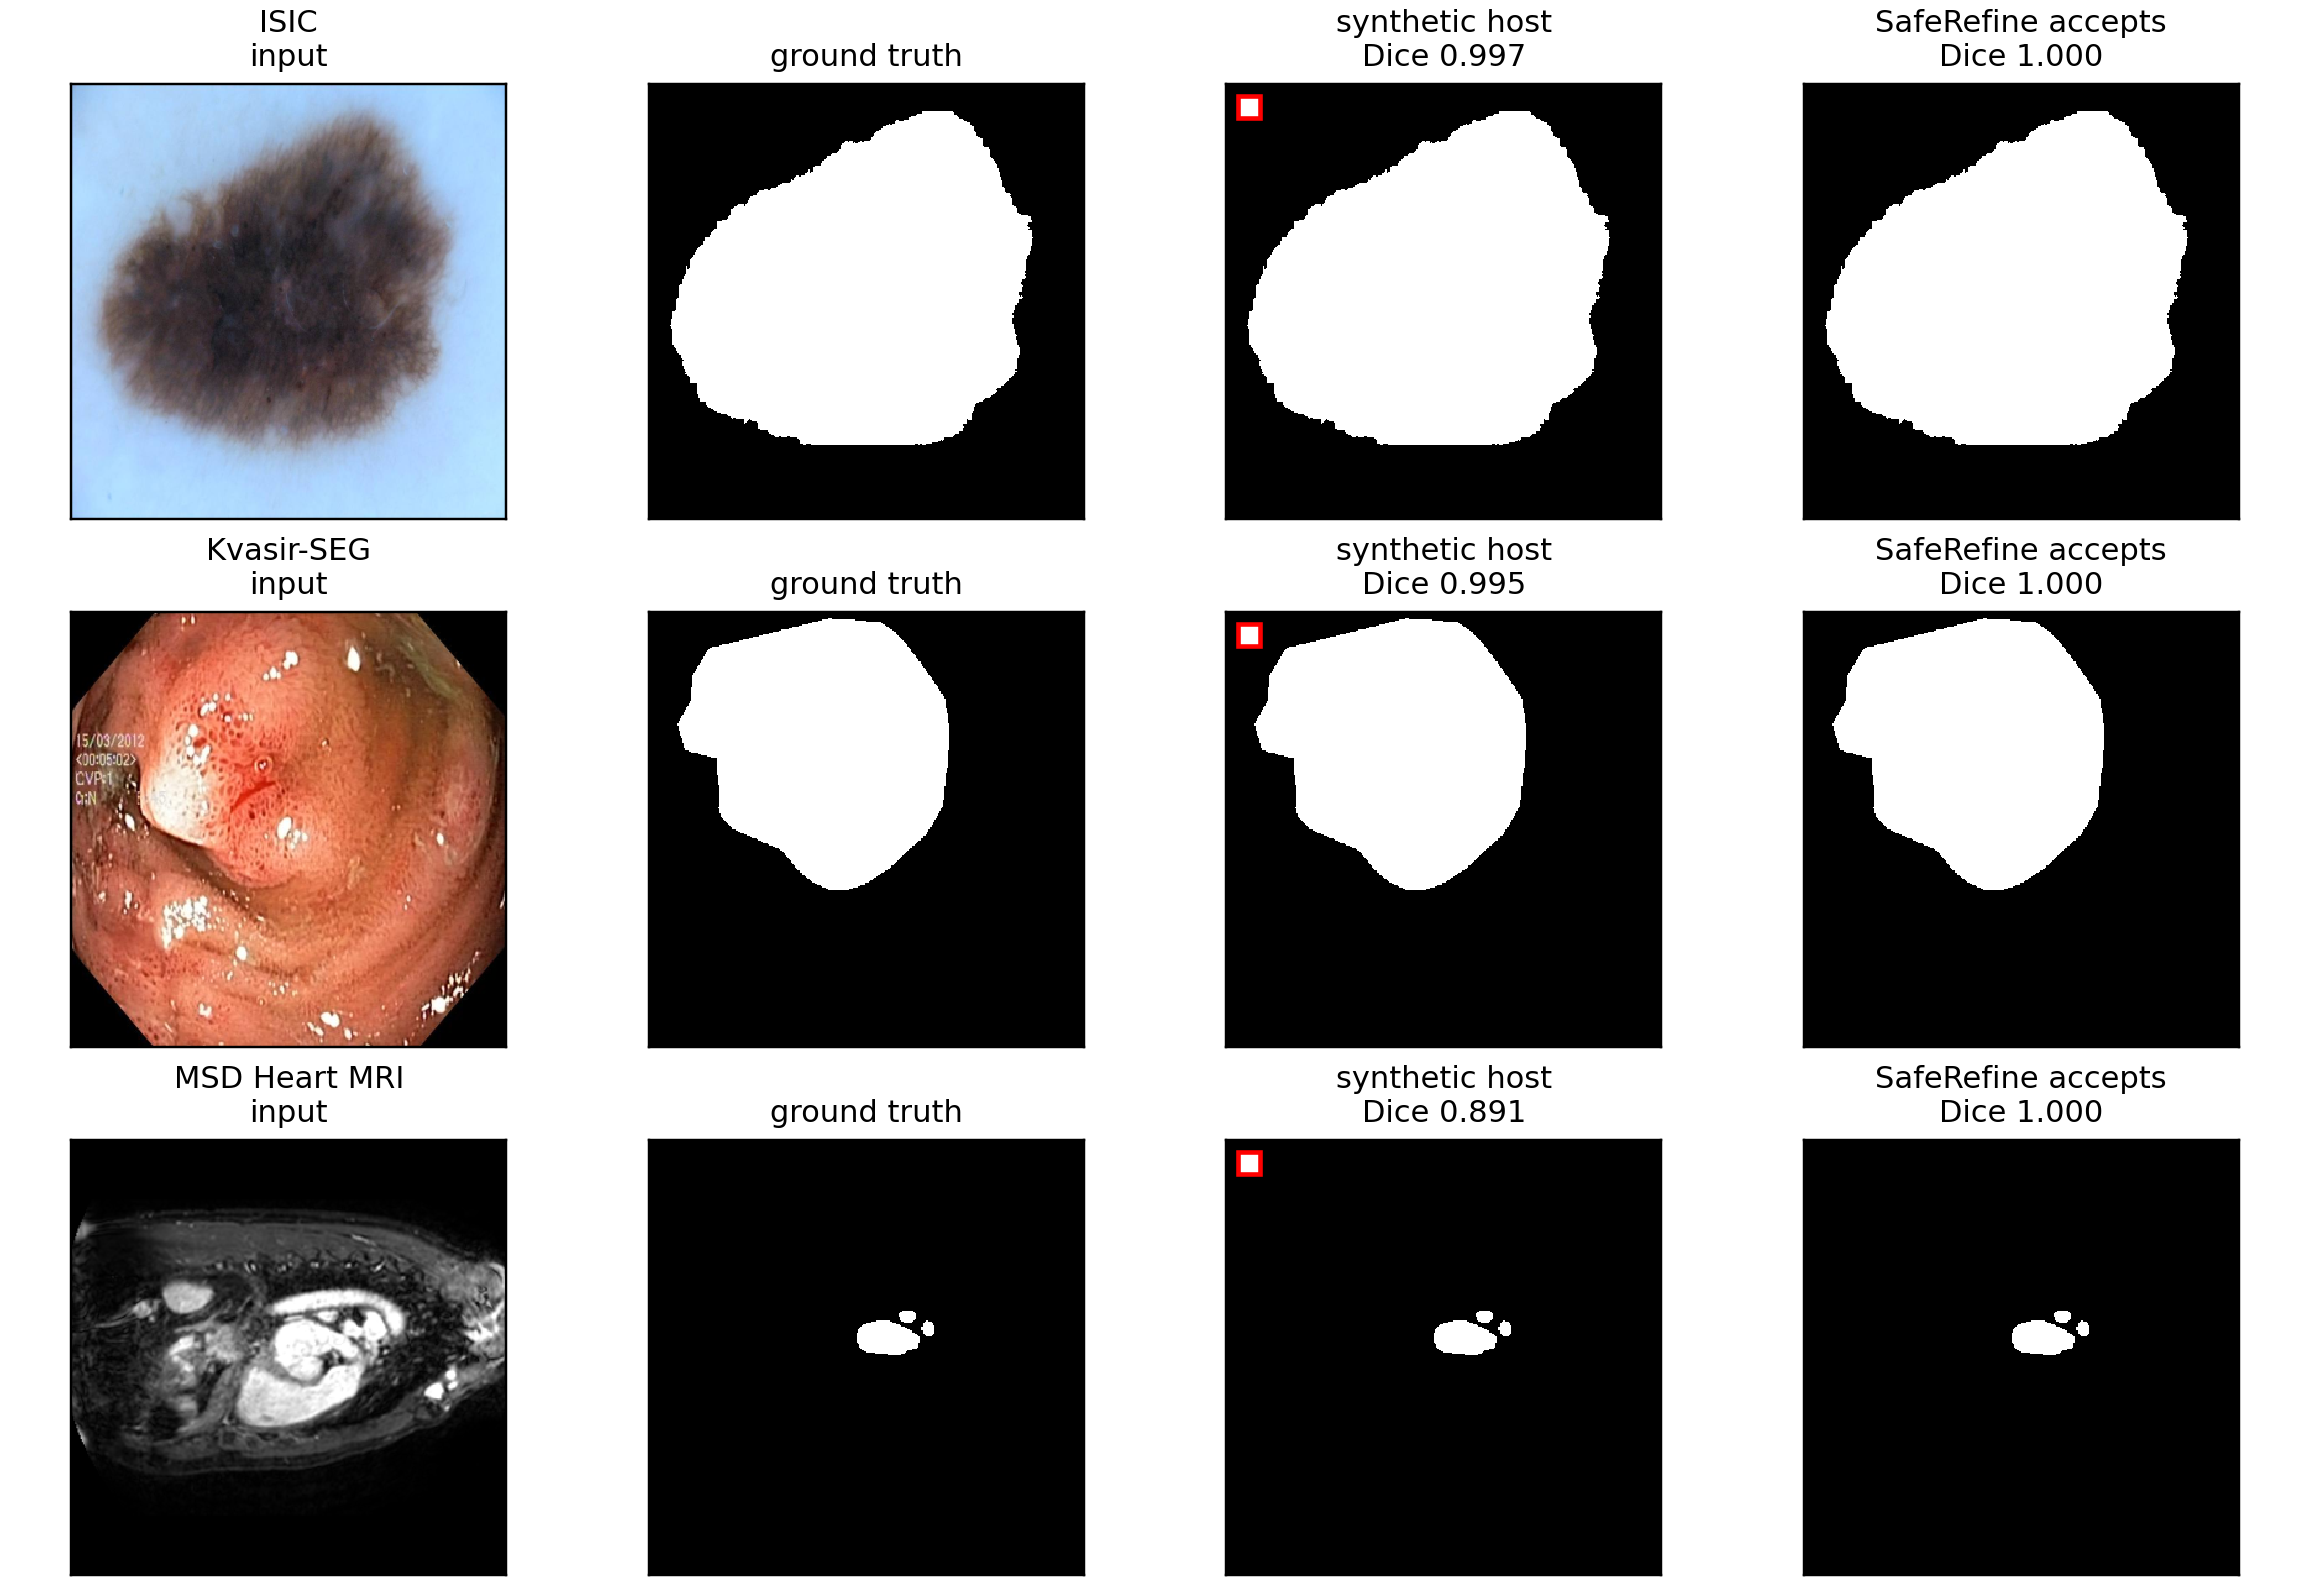
\includegraphics[width=0.95\textwidth]{figures/fig_positive_control_artifact.png}
    \caption{Positive-control artifact-removal sanity check. A synthetic host
    mask is created by adding a known isolated artifact; SafeRefine certifies
    and accepts the artifact-removal refiner, returning the corrected mask. This
    verifies that the method is not intrinsically host-only.}
    \label{fig:positive_control}
\end{figure*}

\subsection{Nested selection reduces multiplicity but does not certify refinement}

A natural concern is that the joint primary policy is too conservative because
the confidence bound pays for the entire action-threshold search space. We
therefore run the nested Bernoulli stress test described above. This reduces
the number of threshold candidates used in the bound from tens of thousands in
the joint portfolio to tens or hundreds after action selection. It also uses
a clinically less brittle harmed event, $g<-0.01$, rather than counting any
infinitesimal Dice decrease.

Even under this more favorable protocol, the certified tail-risk policy still
selects the host in all final settings. The reason is no
longer the global portfolio size alone. Several non-host candidates have
positive calibration gains and low empirical large-drop rates, but the
finite-sample upper bound for the large-drop event remains above the
$\gamma=0.10$ budget. Nested selection therefore strengthens the interpretation
of the primary result: the tested refiners are not certifiable under the stated
tail-risk budgets with the available calibration evidence, even after reducing
the multiplicity penalty and ignoring sub-0.01 Dice changes.
The full nested refusal and non-host diagnostic tables are reported in the
supplement.

\subsection{Certification frontier and sample-size diagnostics}

The nested result at $\gamma=0.10$ does not mean that SafeRefine can never
certify refinement. It means that the specified tail-risk budget is too tight
for the available calibration evidence. Table~\ref{tab:nested_certification_frontier_compact}
varies the large-drop budget while keeping the nested Bernoulli protocol and
$\epsilon=0.01$. At $\gamma=0.05$ and $\gamma=0.10$, no setting certifies a
non-host action. At $\gamma=0.15$, three settings certify intervention; at
$\gamma=0.20$ and $\gamma=0.25$, four and five settings do so, respectively.
This demonstrates that SafeRefine behaves as a certification frontier rather
than a fixed post-processing rule.

The frontier also exposes why a looser budget is not automatically desirable.
Some certified relaxed-budget rows are useful, such as external polyp GraphSeg
at $\gamma=0.15$ with +0.0064 Dice gain and drop05 rate 0.003. Others are poor
deployment choices despite satisfying the looser calibration bound: external
polyp UNet at $\gamma=0.15$ has a worst test drop of -0.6043. We therefore keep
$\gamma=0.10$ as the primary conservative operating point and present larger
budgets only as sensitivity analysis.

\begin{table*}[t]
\centering
\small
\caption{Compact nested Bernoulli certification frontier as the large-drop budget gamma is varied.}
\label{tab:nested_certification_frontier_compact}
\begin{tabular}{lllllllll}
\toprule
setting & gamma & certified & gain & harm & drop\_gt\_0.05 & drop\_gt\_0.20 & worst\_drop & revert\_rate \\
\midrule
ISIC / UNet & 0.05 & no & +0.0000 & 0.0000 & 0.000 & 0.000 & +0.0000 & 1.000 \\
ISIC / UNet & 0.10 & no & +0.0000 & 0.0000 & 0.000 & 0.000 & +0.0000 & 1.000 \\
ISIC / UNet & 0.15 & yes & +0.0017 & 0.0007 & 0.004 & 0.000 & -0.1529 & 0.266 \\
ISIC / UNet & 0.20 & yes & +0.0017 & 0.0007 & 0.004 & 0.000 & -0.1529 & 0.266 \\
ISIC / UNet & 0.25 & yes & +0.0017 & 0.0007 & 0.004 & 0.000 & -0.1529 & 0.266 \\
Kvasir / GraphSeg & 0.05 & no & +0.0000 & 0.0000 & 0.000 & 0.000 & +0.0000 & 1.000 \\
Kvasir / GraphSeg & 0.10 & no & +0.0000 & 0.0000 & 0.000 & 0.000 & +0.0000 & 1.000 \\
Kvasir / GraphSeg & 0.15 & no & +0.0000 & 0.0000 & 0.000 & 0.000 & +0.0000 & 1.000 \\
Kvasir / GraphSeg & 0.20 & no & +0.0000 & 0.0000 & 0.000 & 0.000 & +0.0000 & 1.000 \\
Kvasir / GraphSeg & 0.25 & no & +0.0000 & 0.0000 & 0.000 & 0.000 & +0.0000 & 1.000 \\
Kvasir / UNet & 0.05 & no & +0.0000 & 0.0000 & 0.000 & 0.000 & +0.0000 & 1.000 \\
Kvasir / UNet & 0.10 & no & +0.0000 & 0.0000 & 0.000 & 0.000 & +0.0000 & 1.000 \\
Kvasir / UNet & 0.15 & no & +0.0000 & 0.0000 & 0.000 & 0.000 & +0.0000 & 1.000 \\
Kvasir / UNet & 0.20 & no & +0.0000 & 0.0000 & 0.000 & 0.000 & +0.0000 & 1.000 \\
Kvasir / UNet & 0.25 & no & +0.0000 & 0.0000 & 0.000 & 0.000 & +0.0000 & 1.000 \\
MSD Heart MRI / GraphSeg & 0.05 & no & +0.0000 & 0.0000 & 0.000 & 0.000 & +0.0000 & 1.000 \\
MSD Heart MRI / GraphSeg & 0.10 & no & +0.0000 & 0.0000 & 0.000 & 0.000 & +0.0000 & 1.000 \\
MSD Heart MRI / GraphSeg & 0.15 & no & +0.0000 & 0.0000 & 0.000 & 0.000 & +0.0000 & 1.000 \\
MSD Heart MRI / GraphSeg & 0.20 & no & +0.0000 & 0.0000 & 0.000 & 0.000 & +0.0000 & 1.000 \\
MSD Heart MRI / GraphSeg & 0.25 & yes & -0.0004 & 0.0004 & 0.000 & 0.000 & -0.0259 & 0.984 \\
MSD Heart MRI / UNet & 0.05 & no & +0.0000 & 0.0000 & 0.000 & 0.000 & +0.0000 & 1.000 \\
MSD Heart MRI / UNet & 0.10 & no & +0.0000 & 0.0000 & 0.000 & 0.000 & +0.0000 & 1.000 \\
MSD Heart MRI / UNet & 0.15 & no & +0.0000 & 0.0000 & 0.000 & 0.000 & +0.0000 & 1.000 \\
MSD Heart MRI / UNet & 0.20 & yes & +0.0000 & 0.0001 & 0.000 & 0.000 & -0.0033 & 0.339 \\
MSD Heart MRI / UNet & 0.25 & yes & +0.0000 & 0.0001 & 0.000 & 0.000 & -0.0033 & 0.339 \\
PH2 / UNet & 0.05 & no & +0.0000 & 0.0000 & 0.000 & 0.000 & +0.0000 & 1.000 \\
PH2 / UNet & 0.10 & no & +0.0000 & 0.0000 & 0.000 & 0.000 & +0.0000 & 1.000 \\
PH2 / UNet & 0.15 & no & +0.0000 & 0.0000 & 0.000 & 0.000 & +0.0000 & 1.000 \\
PH2 / UNet & 0.20 & no & +0.0000 & 0.0000 & 0.000 & 0.000 & +0.0000 & 1.000 \\
PH2 / UNet & 0.25 & no & +0.0000 & 0.0000 & 0.000 & 0.000 & +0.0000 & 1.000 \\
Polyp ext. / GraphSeg & 0.05 & no & +0.0000 & 0.0000 & 0.000 & 0.000 & +0.0000 & 1.000 \\
Polyp ext. / GraphSeg & 0.10 & no & +0.0000 & 0.0000 & 0.000 & 0.000 & +0.0000 & 1.000 \\
Polyp ext. / GraphSeg & 0.15 & yes & +0.0064 & 0.0027 & 0.003 & 0.000 & -0.0633 & 0.241 \\
Polyp ext. / GraphSeg & 0.20 & yes & +0.0064 & 0.0027 & 0.003 & 0.000 & -0.0633 & 0.241 \\
Polyp ext. / GraphSeg & 0.25 & yes & +0.0064 & 0.0027 & 0.003 & 0.000 & -0.0633 & 0.241 \\
Polyp ext. / UNet & 0.05 & no & +0.0000 & 0.0000 & 0.000 & 0.000 & +0.0000 & 1.000 \\
Polyp ext. / UNet & 0.10 & no & +0.0000 & 0.0000 & 0.000 & 0.000 & +0.0000 & 1.000 \\
Polyp ext. / UNet & 0.15 & yes & +0.0008 & 0.0116 & 0.043 & 0.000 & -0.6043 & 0.236 \\
Polyp ext. / UNet & 0.20 & yes & -0.0023 & 0.0164 & 0.063 & 0.000 & -0.6043 & 0.141 \\
Polyp ext. / UNet & 0.25 & yes & -0.0023 & 0.0164 & 0.063 & 0.000 & -0.6043 & 0.141 \\
\bottomrule
\end{tabular}
\end{table*}


The external polyp UNet frontier row shows a limitation of controlling only
drop05 rate: a policy can have an acceptable frequency of moderate drops while
still producing a rare severe failure. Table~\ref{tab:nested_severe_certification_frontier_compact}
adds an upper-bound budget of 0.05 on $\Pr(g<-0.20)$ to the nested frontier.
Under this severe-tail constraint, no non-host action is certified even when
the drop05 budget is relaxed to 0.25. This is a deliberately conservative
result, but it clarifies the safety trade-off: preventing rare catastrophic
case-level degradation requires either substantially more calibration evidence
or a different, less distribution-free risk model. The absence of certification
does not imply that every refiner empirically produces severe failures; it means
that the available calibration split is insufficient to certify a bound on rare
catastrophic risk under this distribution-free protocol.

\begin{table*}[t]
\centering
\small
\caption{Severe-tail nested certification frontier with an additional $\Pr(g<-0.20)$ upper-bound budget of 0.05.}
\label{tab:nested_severe_certification_frontier_compact}
\begin{tabular}{lllllllll}
\toprule
setting & gamma & certified & gain & harm & drop\_gt\_0.05 & drop\_gt\_0.20 & worst\_drop & revert\_rate \\
\midrule
ISIC / UNet & 0.15 & no & +0.0000 & 0.0000 & 0.000 & 0.000 & +0.0000 & 1.000 \\
ISIC / UNet & 0.20 & no & +0.0000 & 0.0000 & 0.000 & 0.000 & +0.0000 & 1.000 \\
ISIC / UNet & 0.25 & no & +0.0000 & 0.0000 & 0.000 & 0.000 & +0.0000 & 1.000 \\
Kvasir / GraphSeg & 0.15 & no & +0.0000 & 0.0000 & 0.000 & 0.000 & +0.0000 & 1.000 \\
Kvasir / GraphSeg & 0.20 & no & +0.0000 & 0.0000 & 0.000 & 0.000 & +0.0000 & 1.000 \\
Kvasir / GraphSeg & 0.25 & no & +0.0000 & 0.0000 & 0.000 & 0.000 & +0.0000 & 1.000 \\
Kvasir / UNet & 0.15 & no & +0.0000 & 0.0000 & 0.000 & 0.000 & +0.0000 & 1.000 \\
Kvasir / UNet & 0.20 & no & +0.0000 & 0.0000 & 0.000 & 0.000 & +0.0000 & 1.000 \\
Kvasir / UNet & 0.25 & no & +0.0000 & 0.0000 & 0.000 & 0.000 & +0.0000 & 1.000 \\
MSD Heart MRI / GraphSeg & 0.15 & no & +0.0000 & 0.0000 & 0.000 & 0.000 & +0.0000 & 1.000 \\
MSD Heart MRI / GraphSeg & 0.20 & no & +0.0000 & 0.0000 & 0.000 & 0.000 & +0.0000 & 1.000 \\
MSD Heart MRI / GraphSeg & 0.25 & no & +0.0000 & 0.0000 & 0.000 & 0.000 & +0.0000 & 1.000 \\
MSD Heart MRI / UNet & 0.15 & no & +0.0000 & 0.0000 & 0.000 & 0.000 & +0.0000 & 1.000 \\
MSD Heart MRI / UNet & 0.20 & no & +0.0000 & 0.0000 & 0.000 & 0.000 & +0.0000 & 1.000 \\
MSD Heart MRI / UNet & 0.25 & no & +0.0000 & 0.0000 & 0.000 & 0.000 & +0.0000 & 1.000 \\
PH2 / UNet & 0.15 & no & +0.0000 & 0.0000 & 0.000 & 0.000 & +0.0000 & 1.000 \\
PH2 / UNet & 0.20 & no & +0.0000 & 0.0000 & 0.000 & 0.000 & +0.0000 & 1.000 \\
PH2 / UNet & 0.25 & no & +0.0000 & 0.0000 & 0.000 & 0.000 & +0.0000 & 1.000 \\
Polyp ext. / GraphSeg & 0.15 & no & +0.0000 & 0.0000 & 0.000 & 0.000 & +0.0000 & 1.000 \\
Polyp ext. / GraphSeg & 0.20 & no & +0.0000 & 0.0000 & 0.000 & 0.000 & +0.0000 & 1.000 \\
Polyp ext. / GraphSeg & 0.25 & no & +0.0000 & 0.0000 & 0.000 & 0.000 & +0.0000 & 1.000 \\
Polyp ext. / UNet & 0.15 & no & +0.0000 & 0.0000 & 0.000 & 0.000 & +0.0000 & 1.000 \\
Polyp ext. / UNet & 0.20 & no & +0.0000 & 0.0000 & 0.000 & 0.000 & +0.0000 & 1.000 \\
Polyp ext. / UNet & 0.25 & no & +0.0000 & 0.0000 & 0.000 & 0.000 & +0.0000 & 1.000 \\
\bottomrule
\end{tabular}
\end{table*}


Table~\ref{tab:nested_sample_size_requirement} gives a simple sample-size
diagnostic for the nested $\gamma=0.10$ setting. Holding the empirical drop05
rate and the selected-action threshold count fixed, it reports how many
calibration cases would be needed for the Hoeffding drop05 upper bound to fall
below 0.10. This is an approximate fixed-rate diagnostic, not a formal sample
complexity guarantee: with new calibration data, the empirical drop05 rate, the
selected action, and the number of threshold candidates $M$ could all change.
Even with empirical drop05 equal to zero, Kvasir-SEG GraphSeg would
require roughly 354 calibration cases rather than 38, and external polyp
GraphSeg roughly 425 rather than 200. This supports the interpretation that
the host-only primary result is partly a finite-sample certification result,
not simply a failure of refinement utility.

\begin{table*}[t]
\centering
\small
\caption{Approximate calibration sample size required for the nested best non-host candidate to satisfy the drop05 Hoeffding upper bound at gamma=0.10, holding empirical drop05, M thresholds, and R risk constraints fixed.}
\label{tab:nested_sample_size_requirement}
\begin{tabular}{llllllllllll}
\toprule
setting & risk\_score & cal\_n & M & R & cal\_drop05 & ucb\_drop05 & cal\_drop20 & ucb\_drop20 & required\_n & extra\_n & cal\_gain \\
\midrule
ISIC / UNet & changed & 250 & 207 & 3 & 0.000 & 0.124 & 0.000 & 0.000 & 437 & 187 & +0.0007 \\
Kvasir / GraphSeg & geom & 38 & 39 & 3 & 0.000 & 0.280 & 0.000 & 0.000 & 354 & 316 & +0.0356 \\
Kvasir / UNet & changed & 38 & 37 & 3 & 0.000 & 0.279 & 0.000 & 0.000 & 351 & 313 & +0.0050 \\
MSD Heart MRI / GraphSeg & change\_plus\_geom & 82 & 83 & 3 & 0.000 & 0.202 & 0.000 & 0.000 & 392 & 310 & +0.0000 \\
MSD Heart MRI / UNet & changed & 82 & 30 & 3 & 0.000 & 0.186 & 0.000 & 0.000 & 341 & 259 & +0.0008 \\
PH2 / UNet & change\_plus\_geom & 8 & 4 & 3 & 0.000 & 0.480 & 0.000 & 0.000 & 240 & 232 & +0.0001 \\
Polyp ext. / GraphSeg & changed & 200 & 162 & 3 & 0.000 & 0.136 & 0.000 & 0.000 & 425 & 225 & +0.0135 \\
Polyp ext. / UNet & change\_plus\_geom & 200 & 162 & 3 & 0.015 & 0.151 & 0.000 & 0.000 & 588 & 388 & +0.0175 \\
\bottomrule
\end{tabular}
\end{table*}


Table~\ref{tab:nested_constraint_blockers} complements this sample-size view by
asking what finite-sample budgets would have to be accepted to certify the
highest-gain nested non-host candidate at $\gamma=0.10$. The answer is
setting-specific. ISIC and external polyp GraphSeg are blocked mainly by the
drop05 upper bound, requiring $\gamma_{05}$ values of 0.124 and 0.136,
respectively, rather than the primary 0.10. Kvasir-SEG requires much looser
harmed-rate and drop05 budgets, while PH2 is dominated by its very small
calibration split. External polyp UNet is especially instructive: it has
positive calibration gain but negative test gain and a worst drop of -0.6043,
supporting the severe-tail sensitivity rather than a looser deployment rule.

\begin{table*}[t]
\centering
\small
\caption{Constraint-blocker diagnostics for the highest-gain nested non-host candidate at $\gamma=0.10$. Required budgets are the finite-sample upper bounds that would need to be accepted to certify the candidate; the primary budgets are $\alpha=0.25$ and $\gamma_{05}=0.10$, with $\gamma_{20}=0.05$ in the severe-tail sensitivity.}
\label{tab:nested_constraint_blockers}
\begin{tabular}{lllllllll}
\toprule
setting & risk\_score & cal\_gain & test\_gain & test\_worst & req\_alpha & req\_gamma05 & req\_gamma20 & blocker \\
\midrule
ISIC / UNet & changed & +0.0007 & +0.0018 & -0.0244 & 0.128 & 0.124 & 0.124 & D05 \\
Kvasir / GraphSeg & geom & +0.0356 & +0.0013 & -0.5852 & 0.333 & 0.280 & 0.280 & H,D05 \\
Kvasir / UNet & changed & +0.0050 & +0.0081 & -0.0878 & 0.305 & 0.279 & 0.279 & H,D05 \\
MSD Heart MRI / GraphSeg & host\_uncertainty & +0.0000 & -0.0004 & -0.0259 & 0.202 & 0.202 & 0.202 & D05 \\
MSD Heart MRI / UNet & changed & +0.0008 & +0.0000 & -0.0033 & 0.186 & 0.186 & 0.186 & D05 \\
PH2 / UNet & change\_plus\_geom & +0.0001 & +0.0001 & -0.0006 & 0.480 & 0.480 & 0.480 & H,D05 \\
Polyp ext. / GraphSeg & changed & +0.0135 & +0.0064 & -0.0633 & 0.161 & 0.136 & 0.136 & D05 \\
Polyp ext. / UNet & change\_plus\_geom & +0.0175 & -0.0023 & -0.6043 & 0.176 & 0.151 & 0.136 & D05 \\
\bottomrule
\end{tabular}
\end{table*}


\subsection{Utility-frontier diagnostic}

The primary certified policy returns the host, but this does not mean the
portfolio has no empirical utility. To avoid cherry-picking among relaxed rows,
we define one utility-frontier protocol: under nested action selection, use
$\epsilon=0.01$, require positive calibration-utility fallback, and then
evaluate the selected operating point once on the test split; the full table is
reported in the supplement. This diagnostic
recovers useful rows, including Kvasir-SEG UNet (+0.0081 Dice with 37.8\%
oracle recovery), external polyp GraphSeg (+0.0064 Dice with mean harm
0.0027), and ISIC (+0.0017 Dice). It is not uniformly positive: Kvasir-SEG
GraphSeg has a worst drop of -0.5852, external polyp UNet has negative test
gain with worst drop -0.6043, and MSD Heart MRI GraphSeg has little usable
utility. Thus the portfolio contains useful refinements, but current risk
scores do not reliably identify low-harm interventions under distributional
variation between calibration and test splits.

We therefore treat utility-frontier rows as evidence about available but
uncertified utility. They are diagnostic operating points, not the primary
safety claim and not a safe-improvement mode.

\begin{figure}[t]
    \centering
    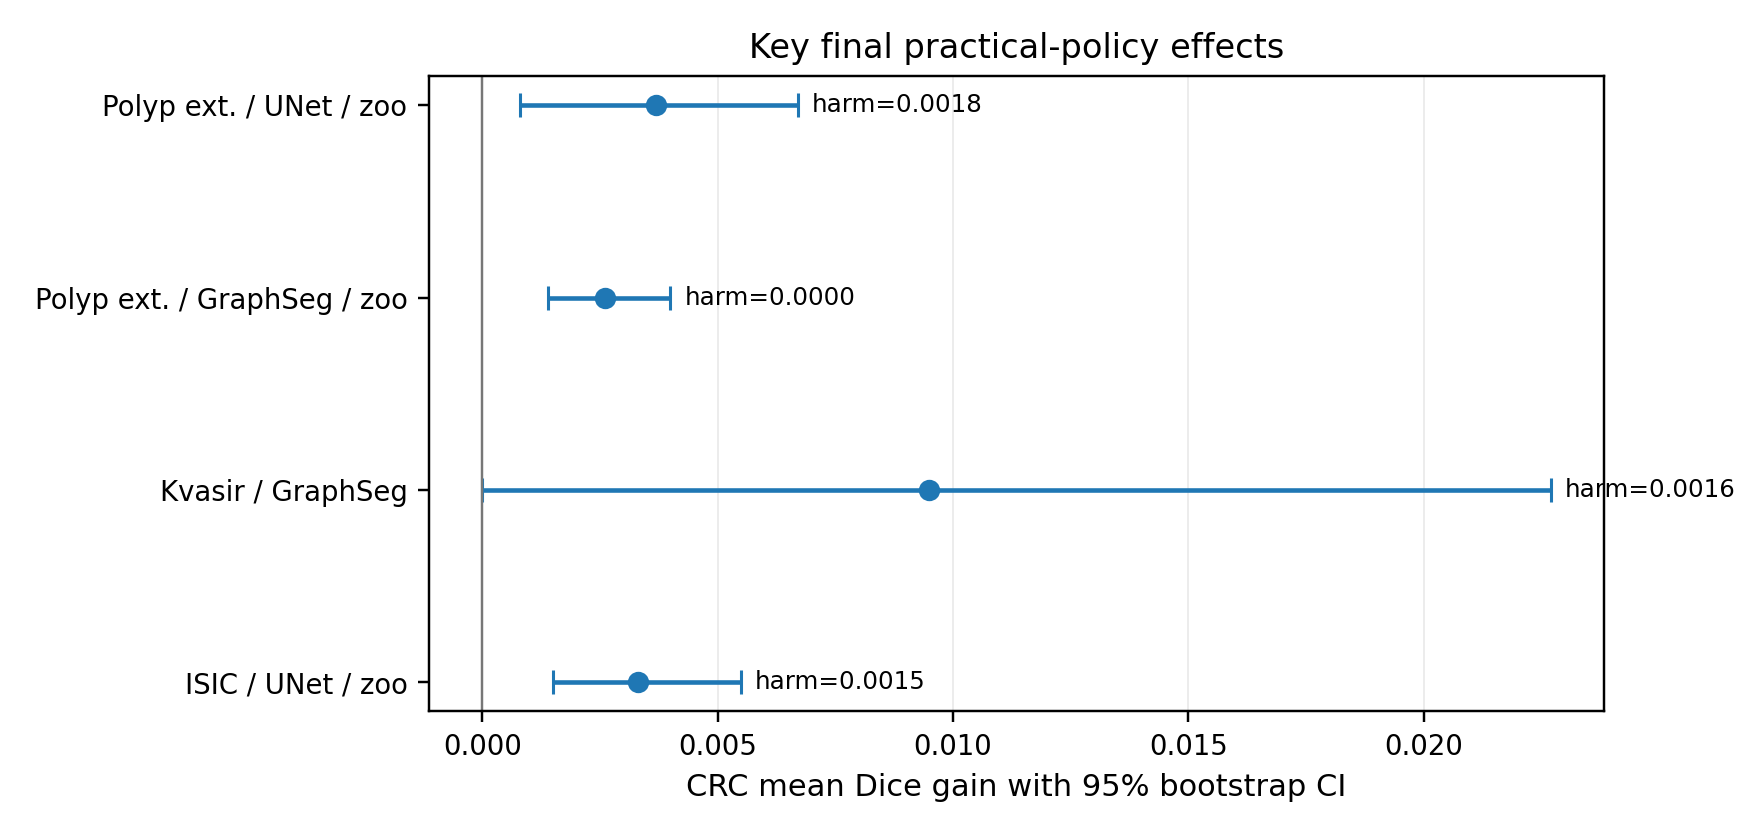
\includegraphics[width=0.95\linewidth]{figures/fig_key_bootstrap_effects.png}
    \caption{Selected relaxed-utility policy effects with 95\% bootstrap
    confidence intervals. These rows summarize diagnostic utility signals and
    should be interpreted alongside the primary tail-risk results, which reject
    all non-host interventions under conservative certification.}
    \label{fig:key_bootstrap}
\end{figure}

\section{Qualitative and Supplementary Diagnostics}

Figure~\ref{fig:case_contactsheet} shows larger qualitative panels for the
main failure mode: a fixed refiner can visibly damage a case, while SafeRefine
returns the host mask. Additional safety-value, decision-baseline,
risk-diagnostic, per-image selection, and full reproducibility tables are moved
to the supplement to keep the main text focused on the certification claim.

\begin{figure*}[t]
    \centering
    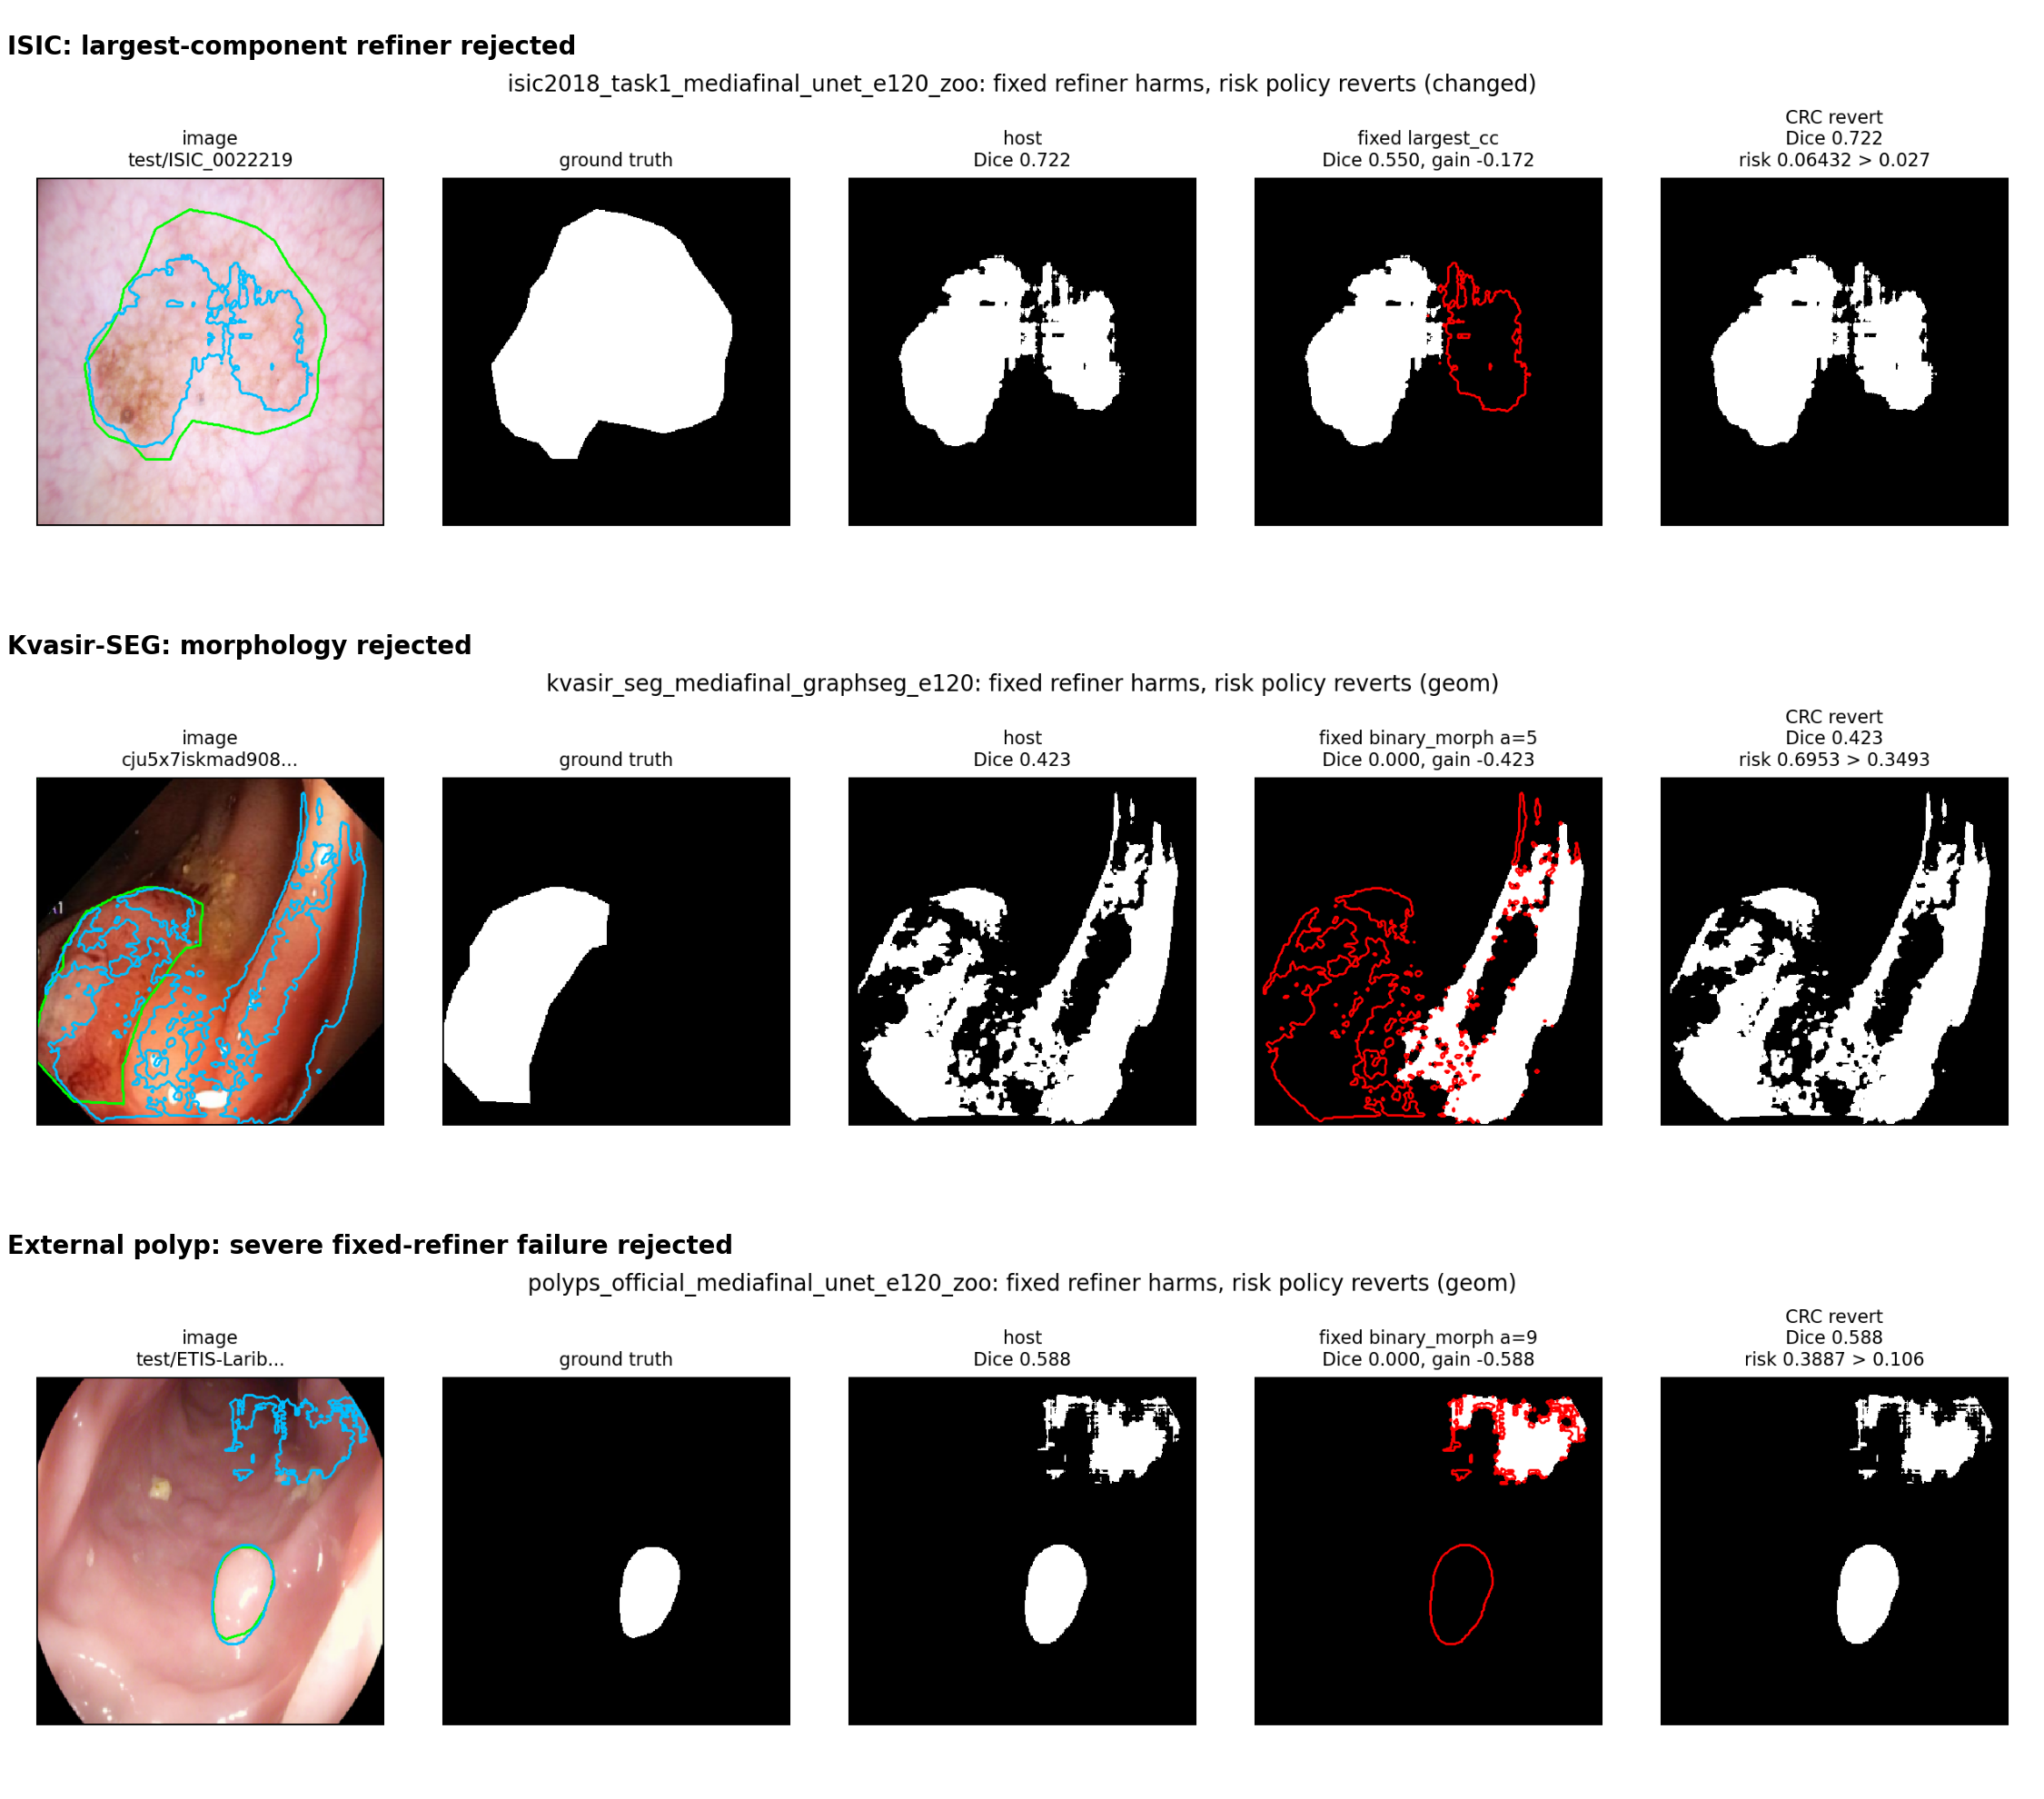
\includegraphics[width=0.95\textwidth]{figures/fig_case_contactsheet.png}
    \caption{Representative mask-level cases where fixed refinement can harm
    and the calibrated controller preserves the host. Each row shows the input,
    ground truth, host prediction, fixed refinement, and SafeRefine output with
    risk-threshold annotation. The ISIC row shows a lesion case where a
    largest-component refiner would reduce Dice and SafeRefine keeps the host;
    the Kvasir row shows morphology collapsing a weak host mask to background;
    the external polyp row shows a morphology action that is attractive on
    average but can damage individual cases. Together with
    Tables~\ref{tab:nested_certification_frontier_compact} and
    \ref{tab:nested_severe_certification_frontier_compact}, these examples
    separate four deployment regimes: host-preserving fallback, refusal of a
    harmful fixed refiner, empirically useful but uncertified refinement, and
    relaxed-frontier acceptance that is rejected once severe-tail risk is
    audited.}
    \label{fig:case_contactsheet}
\end{figure*}

\section{Discussion}

SafeRefine changes how refinement methods should be evaluated. A refiner is not
only a mean-Dice improvement mechanism; it is an intervention that can help,
harm, or be rejected. The host fallback action makes this explicit and gives a
deployment-compatible output even when no non-host refinement is certified.

The method is conservative under tail-risk control and on small calibration
sets. This is a feature rather than a defect for risk-sensitive use: if the
calibration split cannot certify the proposed intervention under harmed-rate,
large-drop, and mean-harm constraints, SafeRefine keeps the host.
Utility-frontier operating points expose where useful refinements may exist,
but those rows should not be read as clinical safety guarantees. In our
results, a predefined utility-frontier protocol is mixed and has low oracle
recovery, while best-case relaxed analyses identify useful refinements in ISIC,
Kvasir-SEG GraphSeg, and external polyp settings. This gap is a limitation of
the current candidate risk scores rather than a result to hide: the portfolio
contains useful refinements, but the tested scores do not reliably recover
oracle utility under safety constraints. The primary tail-risk-controlled
policy preserves the host across all final settings.

The external polyp results are intentionally included as stress tests. We do not
claim that SafeRefine solves external polyp segmentation performance. Instead,
the stress results show that unsafe fixed refiners can be detected or bypassed,
and that broader action portfolios can sometimes identify safer alternatives.

\subsection{Clinical interpretation of host fallback}

SafeRefine is not a clinical safety guarantee. It does not validate the host
model for a clinical indication, does not detect every possible segmentation
failure, and does not replace reader studies or site-specific validation. Its
role is narrower: it can act as a deployment guardrail in pipelines where a
post-hoc refiner is an additional intervention after an already accepted host
model has produced a mask. In that setting, host fallback has a precise
interpretation: if the calibration evidence is insufficient to justify changing
the mask, the deployed output is exactly the same mask the baseline pipeline
would have emitted. The framework therefore formalizes a practical question for
medical segmentation systems: when is it permissible to change a host mask, and
when should the original output be preserved?

\section{Limitations}

SafeRefine is a safety layer around existing segmenters and refiners; it is not
intended to replace strong segmentation backbones. The primary tail-risk policy
can be conservative and may return the host prediction, especially on small
calibration sets or under external shift. Utility-frontier modes can recover
empirical gain but do not eliminate all test-time harm, so worst-drop,
large-drop rate, harmed-rate, and mean harm must be reported. The risk scores
evaluated here are interpretable but imperfect; several are close to random for
harm prediction in some settings, so geometry should not be interpreted as a
universal discovery. SafeRefine should therefore be read as a calibration
framework over imperfect risk scores, not as evidence that any single score
reliably predicts harmful refinement. The current main refiner zoo includes
simple morphology, component, and probability-smoothing operations, plus a
three-setting standalone-segmenter stress portfolio in which an independently
trained UNet is used as an alternative action rather than a host-conditioned
refiner. A benchmark of \emph{conditioned} learned refiners that receive the
host mask or probabilities, for example nnU-Net-style cascades, SAM/MedSAM-guided
mask refinement, SegFix, CascadePSP, or learned boundary/diffusion refiners,
remains an important empirical extension. The
positive-control experiment shows that the controller is not inherently
host-only when a low-risk improving action is available, but the present
clinical stress tests should not be read as evidence that all stronger learned
refiners would fail certification.

\section{Conclusion}

We presented SafeRefine, a model-agnostic tail-risk-controlled refinement
framework for medical image segmentation. By treating refinement as calibrated
acceptance/rejection with exact host fallback, SafeRefine exposes both utility
and harm instead of hiding case-level degradation behind average metrics.
Across multiple medical segmentation settings, hosts, and refiner portfolios,
the primary conservative policy preserves the host when non-host interventions
cannot be certified, while utility-frontier analyses show that useful but
uneven and uncertified empirical utility remains in the portfolio. The
resulting contribution is not clinical deployment safety by itself, nor a
segmentation-improvement method, but a calibrated deployment-time refusal
mechanism for evaluating when segmentation refinement should be accepted and
when the original host output should be preserved.

\section*{Data and Code Availability}

All scripts used to train hosts, evaluate candidate refiners, calibrate action
policies, compute bootstrap confidence intervals, generate figures, and build
paper tables are included in the accompanying repository. Dataset split files,
run manifests, and artifact hashes are provided to support reproducibility.
Public datasets are not redistributed; download/preprocessing scripts and split
definitions are provided where licensing permits.

\section*{Declaration of Competing Interest}

The authors declare that they have no known competing financial interests or
personal relationships that could have appeared to influence the work reported
in this paper.

\section*{CRediT Author Statement}

Author roles will be finalized by the submitting authors.

\section*{Acknowledgements}

Funding, compute, and dataset acknowledgements will be finalized by the
submitting authors.

\bibliographystyle{model2-names}
\bibliography{saferefine_references}

\end{document}
